\documentclass{report}
\usepackage{graphicx}
\usepackage{amsmath}
\usepackage{fancyhdr}
\usepackage{hyperref}
\usepackage{amsthm}
\usepackage{wrapfig}
\usepackage{amssymb}
\usepackage[utf8]{inputenc}
\usepackage[T1]{fontenc}
% \usepackage{geometry}
\usepackage{graphicx}
\newtheorem{theorem}{Theorem}
\usepackage{tikz}
\usetikzlibrary{positioning}
\usetikzlibrary{calc}
\usepackage [ a4paper , hmargin =1.2 in , bottom =1.5 in ] { geometry }
\hypersetup{
    colorlinks=true,
    linkcolor=blue,
    filecolor=magenta,      
    urlcolor=cyan,
}
\pagestyle{fancy}
\lhead{Mathematics of Derivative Pricing}
\rhead{Saksham Rathi}
\fancyfoot[C]{Page Number: \thepage}
%\fancyhf[]{}
\bibliographystyle{plain}
\renewcommand\thesection{\arabic{section}}

\begin{document}

%\title{\textbf{Reinforcement Learning} \\ Summer of Science \\ Mid-Term Report}
%\author{\textbf{Saksham Rathi} \\ \small{Under the mentorship of \textbf{Omar}}}
\begin{titlepage}
\centering
%\pagecolor{yellow}
\vspace*{\fill}

\textbf{\Huge Mathematics of Derivative Pricing} \\
\vspace{0.5cm}
\textbf{\LARGE Summer of Science} \\
\vspace{0.5cm}
\textbf{\Large Report} \\
\vspace{14cm}

\textbf{\LARGE Saksham Rathi}\\
\large Second-Year Computer Science Undergraduate\\
\large 22B1003\\
\large Under the mentorship of \textbf{Shreyas Kulkarni}\\
\end{titlepage}


\tableofcontents

% \clearpage
\section*{Plan of Action}
\addcontentsline{toc}{section}{Plan of Action}
\vspace{1cm}
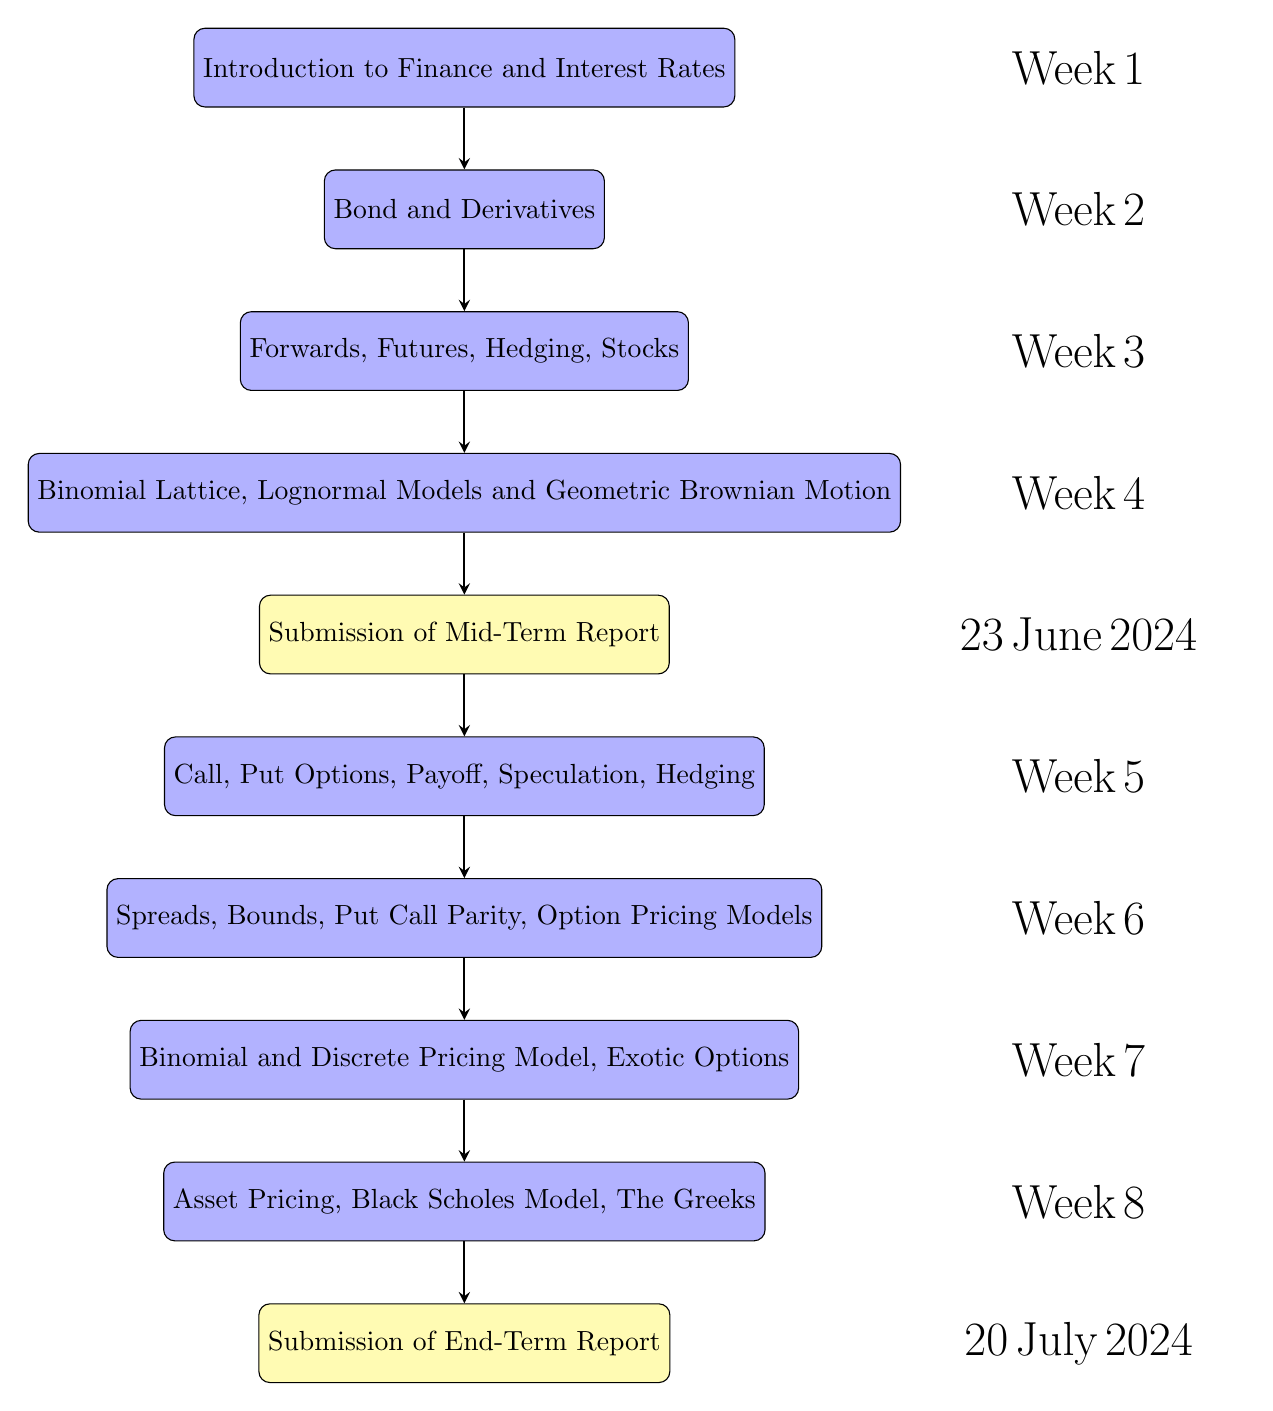
\begin{tikzpicture}[node distance=1.8cm]

% Define styles for different elements
\tikzstyle{action} = [rectangle, rounded corners, minimum width=3cm, minimum height=1cm, text centered, draw=black, fill=blue!30]
\tikzstyle{highlight} = [rectangle, rounded corners, minimum width=3cm, minimum height=1cm, text centered, draw=black, fill=yellow!30]
\tikzstyle{arrow} = [thick,->,>=stealth]
\tikzstyle{interactive} = [text width=4cm, align=center, font=\scriptsize]

% Draw the nodes
\node (start) [action] {Introduction to Finance and Interest Rates};
\node (step1) [action, below of=start] {Bond and Derivatives};
\node (step2) [action, below of=step1] {Forwards, Futures, Hedging, Stocks};
\node (step3) [action, below of=step2] {Binomial Lattice, Lognormal Models and Geometric Brownian Motion};
\node (step4) [highlight, below of=step3] {Submission of Mid-Term Report};
\node (step5) [action, below of=step4] {Call, Put Options, Payoff, Speculation, Hedging};
\node (step6) [action, below of=step5] {Spreads, Bounds, Put Call Parity, Option Pricing Models};
\node (step7) [action, below of=step6] {Binomial and Discrete Pricing Model, Exotic Options};
\node (step8) [action, below of=step7] {Asset Pricing, Black Scholes Model, The Greeks};
\node (step9) [highlight, below of=step8] {Submission of End-Term Report};


% Draw the arrows
\draw [arrow] (start) -- (step1);
\draw [arrow] (step1) -- (step2);
\draw [arrow] (step2) -- (step3);
\draw [arrow] (step3) -- (step4);
\draw [arrow] (step4) -- (step5);
\draw [arrow] (step5) -- (step6);
\draw [arrow] (step6) -- (step7);
\draw [arrow] (step7) -- (step8);
\draw [arrow] (step8) -- (step9);

% Add interactive text
\node [interactive, right of=start, xshift=6cm] {\LARGE Week 1};
\node [interactive, right of=step1, xshift=6cm] {\LARGE Week 2};
\node [interactive, right of=step2, xshift=6cm] {\LARGE Week 3};
\node [interactive, right of=step3, xshift=6cm] {\LARGE Week 4};
\node [interactive, right of=step4, xshift=6cm] {\LARGE 23 June 2024};
\node [interactive, right of=step5, xshift=6cm] {\LARGE Week 5};
\node [interactive, right of=step6, xshift=6cm] {\LARGE Week 6};
\node [interactive, right of=step7, xshift=6cm] {\LARGE Week 7};
\node [interactive, right of=step8, xshift=6cm] {\LARGE Week 8};
\node [interactive, right of=step9, xshift=6cm] {\LARGE 20 July 2024};
\end{tikzpicture}
\clearpage

\section{Introduction to Finance}


In the 1970s, earning around 200 rupees per month was sufficient to comfortably run a 4-member family and have good savings.


In the 1990s, earning around 2000 rupees per month was sufficient to comfortably run a 4-member family, but one can't have good savings.


In the 2010s, earning around 20,000 rupees per month was sufficient just to run a 4-member family, but one can't have savings.


If we talk about today, earning around 20,000 rupees per month is next to impossible to run a 4-member family.


So, if we had kept a 200 rupees note in a cupboard in 1970, then it would be equivalent to 2 rupees in 2020, although the note will physically remain the same. This reduction in the real value is because of "INFLATION".

\begin{figure}[h!]
     \centering
     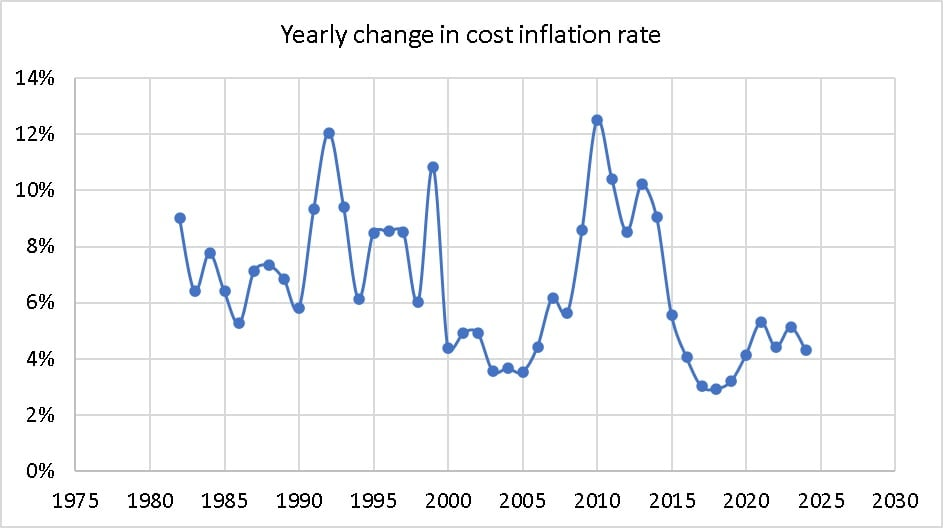
\includegraphics[width=\textwidth]{in.jpg}
     \caption{Yearly change in cost inflation rate in India}
     \label{fig:in}
\end{figure}


Here is a simple equation relating inflation rate(i), real value and nominal value:

\begin{equation}
    \text{Real Value} = \frac{\text{Nominal Value}}{1+\frac{i}{100}}
\end{equation}

So, in the previous scenario, 200 rupees is the nominal value, whereas 2 rupees is the real value.


Investment is the tool to kill inflation.
It can be mainly categorised into two types, namely:
\begin{enumerate}
    \item \textbf{Risk-free Investment} For example: treasury bills (government bonds) and fixed deposit with public sector banks
    \item \textbf{Risky Investment} For example: equity
\end{enumerate}



Let us consider a scenario, where Mr Mohan borrows 100 rupees for his business. In one of the cases, he pays the lender 10 rupees every year to the lender. In another case, he pays the net profit he earns out of his business through the 100 rupees he had borrowed.

The first case is equivalent to bonds and the second case is equivalent to equity/shares. (Where the net profit paid is called dividend)

\subsection{The concepts of Finance Market}
The buying of an asset is called investment.\\Selling an asset and getting back the money is called liquidation.\\Finance market is a platform where we can buy and sell assets that are allowed (listed) by the market. For example: bonds market, equity market, commodity market etc.\\Buyers and sellers are also called traders. Asset get exchanged when both of them agree with each other.\\Every country has atleast one exchange where trades happen. For instance in India, there are two popular exchanges National Stock Exchange (NSE) and Bombay Stock Exchange (BSE).


\subsection{Derivatives Market}
A derivative is a financial contract that derives its value from the price of an underlying asset.


There are various types of derivatives such as forward, future, option and swap. Forward contracts happen over the counter, whereas future contracts happen in a regulatory environment online. In options contract, a marginal price is paid for the contract, but the obligation to execute the contract is removed.


\subsection{Asset Pricing Models}
An investment is an asset.


A simple example of a model is as follows: X is the asset price (principal amount). M is the final amount. r is the rate of interest. Then the following equation links them:
\begin{equation}
    X = \frac{M}{1+r}
\end{equation}


\section{Interest Rates}
The interest in percentage divided by 100 is generally we take as interest rates.

Some useful notations:
\begin{itemize}
    \item $t\longrightarrow$ time
    \item $t = 0 \longrightarrow $ time of investment
    \item $t = T \longrightarrow $ time of maturity
    \item $[0-T] \longrightarrow $ period of investment
    \item Number of times interest is paid during the investment period $\longrightarrow$ frequency in time($n$)
\end{itemize}

If the frequency is n with a constant time interval, interest due times are:
\begin{equation}
    t_k = k\frac{T}{n}
\end{equation}

Let the interest rate be $r$ per annum, then each interest payment will be at the rate $r\frac{T}{n}$.


\subsection{Types of Interest Rates}
\subsubsection{Simple Interest}
\begin{itemize}
    \item $P(0)$ = principle
    \item $r$ = interest rate per annum
    \item $P(T)$ = maturity amount (also called the nominal value)
\end{itemize}

At $t = t_k$, 
\[I_k = P(0)\times r \frac{T}{n}\]
Totally, 
\[
I = \sum_{k=1}^nI_k = P(0)\times rT
\]
\[P(T) = P(0)+I\]
\begin{equation}
    P(T) = P(0)(1+rT)
\end{equation}

\subsubsection{Compound Interest}
The interval $[0-T]$ can be partitioned as $t_0=0$, $t_1 \dots t_n=T$.
At $t=t_1$, 
\[P(t_1) = P(0)(1+\frac{rT}{n})\]
At $t=t_2$, 
\[P(t_2) = P(t_1)(1+\frac{rT}{n})\]
\begin{equation}
\label{ci}
    P(T) = P(0)(1+\frac{rT}{n})^n
\end{equation}

\subsection{Effective Interest Rate}
\begin{equation}
    r_e = \frac{P(T)-P(0)}{TP(0)}
\end{equation}

\subsection{Continuous Compound Interest}
Take the frequency $n\longrightarrow\infty$ in the equation: \ref{ci}.


For any real number $x$:
\[
\lim_{n\rightarrow\infty}(1+\frac{x}{n})^n = e^x
\]


Hence, the nominal value at the continuous compounding interest is given by:
\begin{equation}
    P(T) = P(0)e^{rT}
\end{equation}

\begin{equation}
    \frac{dP}{dt} = rP
\end{equation}


\begin{equation}
    P(t) = P(0) + \int_0^tr(s)P(s)ds 
\end{equation}


The above equation is valid also in the case of time-dependent rates of interest.

\subsection{Present Value}
This means given P(T), we need to find P(0). The procedure of finding the present value for a future amount is called discounting. The present value is often referred to as the discount value. The factor by which the present value P(0) is discounted from the future value is called the discount factor.
\begin{equation}
    D_s = \frac{1}{1+rT}
\end{equation}
\begin{equation}
    D_c = (1+\frac{rT}{n})^{-n}
\end{equation}
\begin{equation}
    D_{cc} = e^{-rT}
\end{equation}


\subsection{Cash Flow Stream}
For a given partition $\{t_0, t_1, \dots, t_n\}$ of a period $[t_0, t_n]$, the cash flow-stream is the (n+1)-tuple $\textbf{x} = (x_0 x_1 \dots x_n)$, where $x_k$ denotes the value of the money transaction occurred at the time $t=t_k$.

\subsection{Future Value of a Stream}
\textbf{Assumption:} Interest rate r (per annum) is constant over $[0-T]$.\\
\textbf{Given:} cash flow stream $\textbf{x} = (x_0 x_1 \dots x_n)$\\
Future value of $\textbf{x}$:\\
For compound interest with frequency n:
\begin{equation}
    FV({\bf x}) = \sum_{k=0}^nx_k(1+\frac{rT}{n})^{n-k}
\end{equation}
For simple interest
\begin{equation}
    FV({\bf x}) = \sum_{k=0}^nx_k(1+r(T-t_k)
\end{equation}
For continuous compound interest:
\begin{equation}
    FV({\bf x}) = \sum_{k=0}^nx_ke^{r(T-t_k)}
\end{equation}
If the cash flow stream is uncountable and is defined by a function f(t). Then the future value for the continuous compound interest scheme is given by:
\begin{equation}
    FV({\bf x}) = \int_0^Tf(t)e^{r(T-t)}dt
\end{equation}

\subsection{Present Value of a Stream}
\textbf{Assumption:} Interest rate r (per annum) is constant over $[0-T]$.\\
\textbf{Given:} cash flow stream $\textbf{x} = (x_0 x_1 \dots x_n)$\\
Present value of $\textbf{x}$:\\

For compound interest with frequency n:
\begin{equation}
    PV({\bf x}) = \sum_{k=0}^n\frac{x_k}{(1+\frac{rT}{n})^{k}}
\end{equation}
For simple interest
\begin{equation}
    PV({\bf x}) = \sum_{k=0}^n\frac{x_k}{(1+rt_k)}
\end{equation}
For continuous compound interest:
\begin{equation}
    PV({\bf x}) = \sum_{k=0}^nx_ke^{-rt_k}
\end{equation}
If the cash flow stream is uncountable and is defined by a function f(t). Then the present value for the continuous compound interest scheme is given by:
\begin{equation}
    FV({\bf x}) = \int_0^Tf(t)e^{-rt}dt
\end{equation}


\subsection{Annuity}
An annuity is a cash flow stream $\textbf{x} = (x_0,  x_1,  \dots,  x_n)$, where
\begin{enumerate}
    \item $sign(x_k)$, for all $k = 1, 2, \dots, n$ are same i.e. all transactions other than the initial one are one-sided (either in-flow or out-flow).
    \item $x_0$ is either 0 or sign($x_0$) is opposite to sign($x_k$), for all $k = 1, 2, \dots, n$.
    \item all transactions are made at equal intervals of time.
\end{enumerate}

\textbf{Example: }instalment payment against purchases, mortgage payments, paying insurance premiums etc.


If the transaction is made at the end of each transaction period $[t_{k-1}, t_k]$, $k = 1, 2, \dots, n$, then the annuity is called the ordinary annuity or annuity-immediate.


\subsection{Internal Rate of Return}
Given a cash flow of stream \textbf{x} = $(x_0 x_1 \dots x_n)$. \\Let us define:
\begin{equation}
\label{rho}
    \rho = \frac{1}{1+\frac{rT}{n}}
\end{equation}

Under compound interest scheme, we have:
\[PV({\bf x}) = x_0 + x_1\rho + \dots + x_n\rho^n\]


IRR Equation:
\begin{equation}
    x_0 + x_1\rho + \dots + x_n\rho^n = 0
\end{equation}
We will calculate the root of this equation and use equation: \ref{rho} to calculate the internal rate of return.



\section{Bond}
A bond is an obligation by the issuer(debtor) to pay money to the holder(creditor) according to a set of rules specified at the time of issue.

\subsection{Zero Coupon Bonds}
Single payment at $t = T$, called a zero-coupon bond or pure discount bond.


\subsection{Coupon Bonds}
Gives a cash flow $(-P_0, C_1, C_2, \dots, C_n+P_n)$ for the holder, where:
\begin{itemize}
    \item each amount $C_k$ is called the coupon value
    \item each such transaction is called the coupon payment
    \item The amount $P_0$ is called the issue price
    \item $P_n$ is called the face value or par value
    \item The rate per annum at which $C_k$ is calculated from $P_n$ is called the $k^{th}$ coupon rate.
\end{itemize}

\subsubsection{Example}
\textbf{Cash Flow:} $b = (0, C, C, \dots, P_n+C)$, where
\begin{itemize}
    \item Each coupon value $C$ is for 1 year and it is paid $m$ times a year.
    \item If the bond duration is $n$ years, then $N=mn$ is the number of times of coupon payment
    \item Take $r$ as the interest rate compounded with frequency $m$ per annum
\end{itemize}

Present value of b:
\begin{equation}
    P_0 = PV(b) = \frac{P_n}{(1+\frac{r}{m})^N} + \sum_{k=1}^N\frac{\frac{C}{m}}{(1+\frac{r}{m})^k}
\end{equation}
The parameter $r$ is called the yield of the bond.


In case of continuous compounding:
\begin{equation}
    PV({\bf b}) = P_ne^{-rn} + \sum_{k=1}^N\frac{C}{m}e^{-rt_k}
\end{equation}


\subsection{Risks}
\begin{itemize}
    \item Credit Risk
    \item Inflation Risk
\end{itemize}


\subsection{Yield to Maturity}
\textbf{First Assumption:} The traded time $t$ is such that $t_k < t < t_{k+1}$, for some k and $t-t_k$ is negligible.

The yield $r(t)$ at the time t (fixed)
\begin{equation}
    P(t) = \frac{P_n}{(1+\frac{r(t)}{m})^{N-k}} + \sum_{j=1}^{N-k}\frac{\frac{C}{m}}{(1+\frac{r(t)}{m})^{j}}
\end{equation}
for the given $P(t)$.\\
$r(t)$ is also called the yield to maturity (YTM).

\subsection{Accrued Interest}
Let the coupon payment is made at $t=t_k$.
Accrued Interest (AI) is calculated using linear interpolation:
\begin{equation}
    AI(t) = \frac{t-t_k}{t_{k+1}-t_k}\frac{C}{m}
\end{equation}

The gross price, denoted by $G(t)$, to be paid by the seller to the buyer is given by:
\begin{equation}
    G(t) = P(t) + AI(t)
\end{equation}

\subsection{Price Sensitivity}
\begin{equation}
    P(r) = \frac{P_n}{(1+\frac{r}{m})^{N-k}} + \sum_{j=1}^{N-k}\frac{\frac{C}{m}}{(1+\frac{r}{m})^{j}}
\end{equation}
As yield increases, the bond price decreases. The function P is convex.

\begin{figure}[h!]
     \centering
     \includegraphics[width=0.5\textwidth]{Screenshot 2024-06-13 at 8.28.56 AM.png}
     \caption{Price vs Yield}
     \label{fig:pvy}
\end{figure}

\subsection{Duration}
The duration of the cash flow stream {\bf x} is defined as:
\begin{equation}
    D({\bf x}) = \frac{\sum_{k=0}^nPV(x_k)t_k}{PV({\bf x})} = \sum_{k=0}^n(\frac{PV(x_k)}{PV({\bf x})})t_k
\end{equation}
\[
D({\bf x}) = \sum_{k=0}^nw_kt_k
\]
\[
\sum_{k=0}^nw_k = 1
\]

Duration when applied to bonds is called {\bf Macaulay Duration}.


\subsection{Price Sensitivity Model}
For any yield $r$ > 0 and $\Delta r > 0$ small, using the mean value theorem, we have
\begin{equation}
    \Delta P = P(r+\Delta r)-P(r) = P'(\rho)\Delta r
\end{equation}
for some $\rho \in (r, r+\Delta r)$


We can write 
\begin{equation}
    P'(r) = -x_j\sum_{j=1}^{N-k}\frac{j}{m}x_j(1+\frac{r}{m})^{-j-1}
\end{equation}
where $x_j = \frac{C}{m}$ for $j = 1, 2, \dots, N-k-1$, and $x_{N-k} = P_n + \frac{C}{m}$.


\begin{equation}
    \Delta P \approx P'(r)\Delta r
\end{equation}

\begin{equation}
\label{ps}
    P'(r) = -D_mPV({\bf b})
\end{equation}
where $D_m = \frac{D({\bf b})}{(1+\frac{r}{m})}$\\

Equation \ref{ps} is called the price sensitivity model.


\section{Derivatives}
A derivative is a contract between two parties that binds a trade between them in an asset, called underlying asset, at a future date called the delivery date or expiration date at some predetermined price of the asset, called strike price.


\subsection{Types of derivatives}
\begin{itemize}
    \item {\bf Contingent Claims:} Are contracts that define the holders the right but not the obligation to execute the contract on or before the expiry. Options are contingent claims.
    \item {\bf Non-Contingent Claims:} Are contracts where both writer and holder have obligation to execute the contract on or before the expiry. Forward, future and swap are non-contingent claims.
\end{itemize}

\subsection{Types of traders}
\begin{itemize}
    \item {\bf Risk Aversion Nature:} quantify the risk involved in the trades, balance it through some alternate trading and investment strategies. Any strategy that is adopted to reduce risk in price fluctuation of an asset is called hedging. A trader with risk aversion nature may be called hedger.
    \item {\bf Risk Seeking Nature:} In contrast a trader with risk seeking nature will take any level of risk to increase their gains. Trading in a risky security with the hope of making profits in a short span of time due to the market fluctuations is called speculation. Traders with risk seeking nature may be called speculators.
\end{itemize}

\section{Forwards}
A forward contract is a non-contingent claim between two parties to buy or sell an asset on the expiration time for a fixed strike price.


Forward trades happen through over the counter (OTC) market.
\subsection{Notations}
\begin{itemize}
    \item Issue time: $t = 0$
    \item Expiration Time: $t=T$
    \item Strike Price/Forward Price: $F(0, T)$
    \item Spot Price: at any time $t \in [0,T]$ is $S(t)$.
    \item Strike price at any time $t \in [0,T]$ is $F(t, T)$.
\end{itemize}


\[
R_F(t; 0, T) := F(t,T)-F(0,T),    t \in [0,T]
\]

\[F(T,T) = S(T)\]


\subsection{Payoff}
The payoff from a forward contract initiated at $t = 0$ is the trader's total return from the contract till expiration, which is given by $R_F(T; 0, T)$ for the long position and $-R_F(T; 0, T)$ for the short position in the contract. 

\subsection{Portfolio}
\begin{itemize}
    \item A collection of risk-free assets is denoted by
    \[{\bf B} = (B_1, B_2, \dots, B_{n_b})\]
    where each $B_i$, $i = 1, 2, \dots, n_b$ is a risk-free asset like a bond.
    \item A collection of risky assets is denoted by
    \[{\bf S} = (S_1, S_2, \dots, S_{n_s})\]
    where each $S_i$, $i = 1, 2, \dots, n_s$ is a risky asset like a stock of a company.
    \item A collection of derivatives is denoted by
    \[{\bf D} = (D_1, D_2, \dots, D_{n_d})\]
    where each $D_i$, $i = 1, 2, \dots, n_d$ is one of the derivative instruments.
\end{itemize}


A portfolio is a collection of assets $({\bf B, S, D}))$ is an ordered $(n_b + n_s + n_d)$-tuple of real numbers
\[\Pi := ({\bf b, s, d})\]
where ${\bf b} = (b_1, \dots, b_{n_b}$ with $b_i$ being the number of asset $B_i$ (and similarly).


Building a portfolio consists of three steps:
\begin{enumerate}
    \item Select the assets to be collected in the portfolio and their quantities
    \item Plan the order in which they have to be traded (sometime this ordering may not matter)
    \item Trade (buy and sell) the assets in the market as planned
\end{enumerate}

\subsection{Portfolio Value}
Assume that a portfolio is built at $t = 0$ and is held till $t = T$. The portfolio value at any time $t \in [0,T]$ is defined as:
\begin{equation}
    V(\Pi)(t) = \sum_{i=1}^{n_b}b_iB_i(t) + \sum_{i=1}^{n_s}s_iS_i(t) + \sum_{i=1}^{n_d}d_iD_i(t)
\end{equation}

\subsection{Arbitrage Portfolio}
\begin{enumerate}
    \item $V(\Pi)(0) = 0$
    \item $V(\Pi)(T) \geq 0$
    \item \( \mathbb{P}(V(\Pi)(T) > 0) > 0 \)
\end{enumerate}

\subsection{Theorem: No-cost Forward Pricing}
Suppose the underlying asset has no extra cost involved throughout the forward contract period. Further assume that there is no arbitrage opportunity available in the market and the market allows short trades.


Then, the forward price at any time $t \in [0,T]$ is given by
\begin{equation}
F(t,T) = \begin{cases} 
S(t)(1+\frac{r}{m})^n - AI(t) & \text{for discrete compounding}\\
S(t)e^{r(T-t)} & \text{for continuous compounding } 
\end{cases}
\end{equation}


\subsection{Forward Pricing (with cost) model}

Assume that the underlying asset involves an additional cost of Rs. $C$ to maintain during the forward contract period $[0-T]$. Further assume that there is no arbitrage opportunity available in the market and the market allows short trades.


Then, the fair forward price is given by
\begin{equation}
F(0,T) = (S(0)+C)e^{rT}
\end{equation}

\subsection{Forward Pricing (with dividend yield) model}

Assume that the underlying asset pays dividend continuously at the rate $r_d$. Further assume that there is no arbitrage opportunity available in the market and the market allows short trades.


Then, the fair forward price is given by
\begin{equation}
F(0,T) = S(0)e^{(r-r_d)T}
\end{equation}


\subsection{Forward Pricing (with dividend) model}

Assume that the underlying asset pays dividend $x$ rupees at time $t = \tau \in [0,T]$. Further assume that there is no arbitrage opportunity available in the market and the market allows short trades.


Then, the fair forward price is given by
\begin{equation}
F(0,T) = (S(0)-xe^{-r\tau})e^{-rT}
\end{equation}


\subsection{Value of Forward Contract}
Assume that there is no arbitrage opportunity available in the market and the market allows short trades.


Then the value of a long forward contract at any time $t \in [0,T]$ is given by
\[
V(t) = (F(t,T)-F(0,T))e^{-r(T-t)}
\]

The value of a short forward contract is given by $-V(t)$.



\section{Swap}
A swap is another type of non-contingent derivative contract where cash flow streams are exchanged through OTC between two parties over a series of specified future dates according to certain specified rules.


\section{Futures}
They are another type of non-contingent claims. They are very much similar to forward contracts.


Forward contracts are OTC (over the counter), whereas futures happen through exchanges (for example: NSE, BSE). In case of forward, the contract gets settled on the expiration date only, whereas futures are setting through marking to market concept.

\subsection{Marking to Market}
Exchange collect some margin deposit from both the parties. If the contract was initiated on day-0, then on day-1, party-A (long position) will pay $f(1, T)- f(0, T)$ and party-B (short position) will pay $f(0, T)- f(1, T)$, and this process will continue.


\subsection{Future Pricing}
Future price at $t$ is $f(t, T)$. The time at which a contract is initiated is taken at $t = 0$. The future period is $[0, T]$ where $T$ is the expiration time.


If long and shorts are allowed with fractional units and there are no arbitrage opportunities.


If the prevailing interest rate is constant for the period $[0, T]$ of the future then:
\[f(t, T) = F(t, T)\]

\section{Hedging}
The primary use pf futures contracts is to hedge our investments against risks.


In a perfect hedging, an investor's risk in a future commitment to deliver or receive an asset is completely eliminated by taking an equal and opposite position in the futures market, if such an opportunity is available.


\subsection{Minimum-Variance Hedging}
Suppose the number of trading units is $N$ (negative if a long position, else positive).
$h$ is the position taken in the future contract with future price $f(0, T)$. 
\[C = V + (f(\tau, \tau) - f(0, \tau))h\]

Our aim is to minimize the risk by appropriately choosing $h$. ($C$ = cash received.)
Risk associated is the standard deviation of the random variable $C$.


\begin{equation}
    Var(C) = Var(V) + 2hCov(V, f(\tau, \tau)) + h^2Var(f(\tau, \tau))
\end{equation}

The minimum of Var(C) is at
\[
h = -\frac{Cov(V, f(\tau, \tau))}{Var(f(\tau, \tau)}
\]


\section{Stocks}
\begin{figure}[h!]
     \centering
     \includegraphics[width=\textwidth]{Screenshot 2024-06-20 at 10.33.23 PM.png}
     \label{fig:csb}
\end{figure}

\subsection{Stock Price Behaviour}
When the business prospects of the company improve, profit prospects improve and the outlook for future dividends improves. As a result, the share price will increase.


\subsection{Efficient Market Hypothesis}
The current price of a stock reflects all available information and will only change with the arrival of new information.

\section{Binomial Lattice Model}
Let the present price of the stock as $S_0$. Take the holding period as $[0, \infty)$.


In the interval, $[t_k, t_{k+1}]$ we will apply the one-step binomial model. Let the stock price be $S_k$ at $t_k$. Let $r_k$ be the interest rate during that period.


No arbitrage condition:
\[d_k < (1+r_k) < u_k\]


$S_k = \{d_k, u_k\}$ $\sigma $field in the power set. The discrete probability is $\mathbb{P}(u_k)= p_k$. Define the random variable $x_{k+1}(s) = S_ks$.


\[S_{k+1} = X_{k+1}\]


The probability $p$ is given by the fair game criteria. The expected present value should be equal to $S_0$.


\subsection{Risk-neutral probability}
For continuous compounding:
\begin{equation}
    p = \frac{e^{rT}-d}{u-d}
\end{equation}

Based on the fair game criteria.


\subsection{Multi-step Binomial Lattice Model}
One can apply one-step binomial lattice model sequentially.
\begin{figure}[h!]
     \centering
     \includegraphics[width=\textwidth]{Screenshot 2024-06-22 at 9.18.18 AM.png}
     \caption{Two-Step Binomial Lattice Model}
     \label{fig:tblm}
\end{figure}


\section{Lognormal Model}
We need to find stock prices at any future time. And, we need to move from discrete time model to continuous time model.

We assume the form:
\[S(t) = S_0e^{R(t)}\]
where $R(t)$ is a random variable.

As time $t_k$, we propose the stock price to be 
\[S(t_{k+1}) = S_{t_k}e^{R(t_k)}\]

\[S(1) = \frac{S(t_n)}{S(t_{n-1})} \times \frac{S(t_{n-1})}{S(t_{n-2})} \times \dots \times \frac{S(1)}{S_0}\
\]


\[S(1) = S_0 exp(\sum_{k=0}^{n-1}R(t_k))\]
\[ln(\frac{S(1)}{S_0}) = \sum_{k=0}^{n-1}R(t_k) \]


We assume that $R(t_k)$ are mutually independent and identically distributed. 
\[\mathbb{E}(ln(\frac{S(1)}{S_0})) = \mu = n\Tilde{\mu}\]

\[\sigma^2 = Var(ln(\frac{S(1)}{S_0})) = n\Tilde{\sigma}^2\]

We can apply Central Limit Theorem.


\[
\frac{ln(\frac{S(1)}{S_0})-\mu}{\sigma} \rightarrow \mathbb{N}(0, 1)
\]


In lognormal model, we assume 
\[S(T) = S_0e^R\]
$\frac{S(T)}{S_0)}$ is lognormally distributed with parameters $T\mu$ and $T\sigma^2$, where $\mu$ and $\sigma^2$ are mean and variance of 1-year stock price S(1).



\begin{equation}
    \mathbb{E}(S(T)) = S_0e^{(\mu+\frac{\sigma^2}{2})T}
\end{equation}

\begin{equation}
    Var(S(T)) = S_0^2e^{(2\mu+\sigma^2)T}(e^{\sigma^2T}-1)
\end{equation}


\section{Geometric Brownian Motion}
Define:
\[W(t) = \frac{ln(\frac{S(T)}{S_0})-t\mu}{\sigma}\]

$\{W(t) | t\in [0,T]\}$ is a stochastic process and satisfies the following properties:
\begin{enumerate}
    \item W(0) = 0
    \item $\mathbb{E}(W(t)) = 0$
    \item $Var(W(t)) = t$
    \item $W(t_1), W(t_2) - W(t_1), \dots, W(t_n) - W(t_{n-1})$ are independent.
    \item The map $t \rightarrow W(t)$ is a continuous process.
\end{enumerate}

Hence, $\{W(t) | t\in [0,T]\}$ is a Brownian Motion.
We can write:
\begin{equation}
    S(t) = S_0exp(t\mu + \sigma W(t))
\end{equation}

Such a process is called a geometric brownian motion with parameters $\mu$(drift) and $\sigma$(volatility).


\section{Options}
Options are contingent claims where the writer has obligation but the holder has only right but no obligation to exercise the contract.


The holder has to pay premium at the time of agreeing for the contract. The premium is called the price of the option or option price.


\subsection{Types of Options}
\begin{itemize}
    \item \textbf{Call Option:} A call option gives the holder of the option the right to buy the underlying asset for a strike price by a certain date.
    \item \textbf{Put Option:} A call option gives the holder of the option the right to sell the underlying asset for a strike price by a certain date.
\end{itemize}

Basic Parameters:
\begin{itemize}
    \item contract issued time, generally taken as t=0
    \item expiration or maturity (date or time), denoted by $t=T$
    \item strike price or exercise price, denoted by $S_T$
    \item contract size also called a lot, which is the number of units of the underlying asset to be exercised in a contract
\end{itemize}


\subsection{Categorization of Options}
\begin{itemize}
    \item In American option, the contract can be exercised at any time up to the expiration time
    \item In European option, the contract is allowed to be exercised only on the expiration date
\end{itemize}


\subsection{Payoff and Gain}
\begin{itemize}
    \item $S_t = S(t): $the current market price of the underlying asset
    \item $K$: strike price of the option
    \item $T$: expiration time
    \item $[0,T]$: the period of the option
\end{itemize}


\begin{itemize}
    \item The owner of a call option will exercise it if and only if $K < S_t$
    \item The owner of a put option will exercise it if and only if $K > S_t$
\end{itemize}


A call option is said to be:
\begin{enumerate}
    \item in-the-money if $K < S_t$
    \item at-the-money if $K = S_t$
    \item out-of-the-money if $K > S_t$
\end{enumerate}


The payoff of a call option at the expiration date is defined as:
\[
C_T = max(0, S_T-K)
\]

The payoff of a put option at the expiration date is defined as:
\[
P_T = max(0, K-S_T)
\]


The value of a call option is defined as:
\[
C_t = max(0, S_t-K)
\]

The payoff of a put option is defined as:
\[
C_t = max(0, K-S_t)
\]

The gain (or loss) is defined as:
\[G_T = C_T - Xe^{rT}      \text{(for long call)}\]
\[G_T = Xe^{rT} - C_T      \text{(for short call)}\]


\section{Spreads}
A spread is a portfolio consisting of options of the same type (either all calls or all puts).
\begin{itemize}
    \item A vertical spread is a portfolio in which the options have the same expiration date, but different strike prices.
    \item A horizontal spread is a portfolio in which the options have the same strike price but different expiration dates
    \item A diagonal spread is a portfolio in which the options have different expiration dates and different strike prices.
\end{itemize}



\subsection{Bull Spread}
Buying a call option at $K_1 - strike$ and writing another call option of the same type at $K_2-strike$ with same expiration and $K_1 < K_2$, leads to a bull spread.

\subsection{Bear Spread}
Buying a put option at $K_2 - strike$ and writing another put option of the same type at $K_2-strike$ with same expiration and $K_1 < K_2$, leads to a bull spread.

\subsection{Butterfly Spread}
Let $K_1 < K_2 < K_3$ and $K_2 \in [S_0-\epsilon, S_0+\epsilon]$ for some sufficiently small $\epsilon > 0$. Buy two call options, one in each of $K_1-strike$ and $K_3-strike$. Write two call options with $K_2-strike$. All options have the same expiration. The resulting portfolio is called the butterfly spread.


\section{Bounds for European Options}
Consider the European call option:
\begin{itemize}
    \item K-strike
    \item period [0,T]
    \item premium $C^e$
\end{itemize}

where the underlying stock with spot price $S_0$ pays no dividend during the option period. If the market does not allow arbitrage, then:
\[max(0, S_0-Ke^{-rT}) \leq C^e \leq S_0\]
where $r$ is the prevailing annual interest rate continuously compounded.


Consider the European put option:
\begin{itemize}
    \item K-strike
    \item period [0,T]
    \item premium $P^e$
\end{itemize}

where the underlying stock with spot price $S_0$ pays no dividend during the option period. If the market does not allow arbitrage, then:
\[max(0, Ke^{-rT}-S_0) \leq P^e \leq Ke^{-rT}\]
where $r$ is the prevailing annual interest rate continuously compounded.



Consider the European (put or call) option:
\begin{itemize}
    \item K-strike
    \item period [0,T]
    \item premium $C^e$ for call and $P^e$ for put,
\end{itemize}

where the underlying stock with spot price $S_0$ pays a dividend $D_0$ at some time during the option period. If the market does not allow arbitrage, then:
\[max(0, S_0-Ke^{-rT}-D_0) \leq c^e \leq S_0-D_0\]
\[max(0, Ke^{-rT}+D_0-S_0) \leq P^e \leq Ke^{-rT}\]
where $r$ is the prevailing annual interest rate continuously compounded.



\section{Bounds for American Options}
Consider two call options:
\begin{itemize}
    \item K-strike call
    \item period [0,T]
    \item premium $C^e$ for the European and $C^a$ for the American
\end{itemize}

If the underlying stock does not pay dividend during the option period, the market does not allow arbitrage, and the prevailing interest rate $r > 0$, then show that $C^e = C^a$.


Consider the American call option:
\begin{itemize}
    \item K-strike
    \item period [0,T]
    \item premium $C^a$
\end{itemize}

where the underlying stock with spot price $S_0$ pays no dividend during the option period. If the market does not allow arbitrage, then:
\[max(0, S_0-Ke^{-rT}) \leq C^a \leq S_0\]
where $r$ is the prevailing annual interest rate continuously compounded.


Consider the American put option:
\begin{itemize}
    \item K-strike
    \item period [0,T]
    \item premium $P^a$
\end{itemize}

where the underlying stock with spot price $S_0$ pays no dividend during the option period. If the market does not allow arbitrage, then:
\[max(0, K-S_0) \leq P^a \leq K\]
where $r$ is the prevailing annual interest rate continuously compounded.


Consider the American (put or call) option:
\begin{itemize}
    \item K-strike
    \item period [0,T]
    \item premium $C^a$ for call and $P^a$ for put,
\end{itemize}

where the underlying stock with spot price $S_0$ pays a dividend $D_0$ at some time during the option period. If the market does not allow arbitrage, then:
\[max(0, S_0-Ke^{-rT}-D_0, S_0-K) \leq c^a \leq S_0\]
\[max(0, Ke^{-rT}+D_0-S_0, K-S_0) \leq P^a \leq K\]
where $r$ is the prevailing annual interest rate continuously compounded.


\section{Put-Call Parity Estimates}
Consider the two European options:
\begin{itemize}
    \item K-strike
    \item period [0,T]
    \item premium $C^e$ for the call option and $P^e$ for the put option
\end{itemize}

where the underlying stock with spot price $S_0$ pays no dividend during the option period. If the market does not allow arbitrage, then:
\[C^e - P^e = S_0 - Ke^{-rT}\]
where $r$ is the prevailing annual interest rate continuously compounded.


Consider the two American options:
\begin{itemize}
    \item K-strike
    \item period [0,T]
    \item premium $C^a$ for the call option and $P^a$ for the put option
\end{itemize}

where the underlying stock with spot price $S_0$ pays no dividend during the option period. If the market does not allow arbitrage, then:
\[S_0-K \leq C^e - P^e \leq S_0 - Ke^{-rT}\]
where $r$ is the prevailing annual interest rate continuously compounded.


\section{Premium Properties}
If the underlying stock does not pay dividend during the option period and the market does not allow arbitrage, then
\[0 \leq C^e(K_1) - C^e(K_2) \leq e^{-rT}(K_2-K_1)\]
\[0 \leq P^e(K_2) - P^e(K_1) \leq e^{-rT}(K_2-K_1)\]
for any $0 \leq K_1 \leq K_2$, where $r$ is the prevailing interest rate continuously compounded and all the options have the same period [0,T]


For any $\alpha \in [0,1]$ and for any positive real numbers $K_1$ and $K_2$, we have:
\[C^e(\alpha K_1 + (1-\alpha)K_2 \leq \alpha C^e(K_1) + (1-\alpha)C^e(K_2) \]
\[P^e(\alpha K_1 + (1-\alpha)K_2 \leq \alpha P^e(K_1) + (1-\alpha)P^e(K_2) \]
where all the options have the same expiration and market does not allow arbitrage.


\section{Discrete Time Pricing Model}
Let the period of the option be [0,T]. $t_k = kh$ where $h = \frac{T}{n}$. At $t = t_k$ the stock price in the spot market be denoted as $S(t_k)$.


In general, at $=t_k$ we know $S_k$ and for $S_{k+1}$. We only know $S_k$ which is $U$ or $D$.

Let $S = \{s = (s_1, s_2, \dots, s_n) | s_k \texttt{is either U or D}\}$


\[B_{s_k} = \{s \in S | \texttt{the first k components of s} = s_k \}\]



\subsection{Filtration}
A collection $\{F_t | t \geq 0\}$ of $\sigma$-fields on $S$ is called a filtration if 
\[F_s \in F_t\]
for all $0 \leq s \leq t$


\subsection{Trading Strategy}
Our portfolio $\pi = (\phi, \theta)$, $\phi$ is a scalar and $\theta$ is a vector.


The stochastic process of portfolios
\[\{\Pi_k | k = 1, \dots, n\}\]
where $\Pi_k$ corresponds to the period $[t_{k-1}, t_k]$ is called a trading strategy, if each component of $\Pi_k$ is $F_{k-1}$ is measurable.


\subsection{Value Process}
For $k = 0, 1, \dots, n$, let $S_k = (S_k^1, \dots, S_k^m)$ be the price vector at time $t = t_k$ , where $S_k^j$ denotes the price of the $j^{th}$, risky asset at $t=t_k$ We also denote the risk-free asset price at $t = t_k$ as $B_k$. The stochastic process $\{V_k | k = 1, \dots, n\}$ where

\begin{equation}
    V_k = \phi B_k + \theta_k.S_k
\end{equation}
is the value of the portfolio $\Pi_k$ is called the value process or the wealth process.

\subsection{Discounted Finance Market}
\[B = \{B_k\}, B_k > 0\]
\[\tilde{S_k} = \frac{S_k}{B_k}\]
Finance Market: $(1, \tilde{S_k})$


\subsection{Self-Financing Trading Strategy}
A trading strategy is called self-financing trading strategy if 
\[V(\Pi_k)(t_k) = V(\Pi_{k+1})(t_k)\]
for every $k = 1, 2, \dots, n-1$


For a discounted finance market, 
$\Delta \phi_k + \Delta \theta_k . \tilde{S_k} = 0$


\subsection{Replicative Strategy}
An option is said to be attainable (or reachable) if there exists a self-financing trading strategy, whose value process satisfies:
\[V_n = H_T\]
A trading strategy that makes an option attainable is called a replicative strategy (or a headging strategy).


In market, if every option is attainable, then the market is said to be complete.



\section{One-Step Binomial Model}
The method consists of two steps: 
\begin{enumerate}
    \item Constructing a replicative strategy using the :
    $V_1 = H_T = max(0, S_T-K) \texttt{or} max(0, K-S_T)$ for call and put options respectively
    \item Matching the initial investment: The amount spent in setting up the replicative portfolio at t=0 should be taken as the option premium.
\end{enumerate}


\section{n-step Method (Backward Induction Technique)}
We consider a European option with payoff $H_T$


Given the $\mathbb{F}_{n-1}$-measurable random variable $S_{n-1}$, define
\[
S_n = 
\begin{cases}
    S_{n-1}u & \text{if } s_n = U \\
    S_{n-1}d & \text{if } s_n = D \\
\end{cases}
\]

Then the payoff is given by:
\[
H_n = \begin{cases}
    H_n^u & \text{if } s_n = U \\
    H_n^d & \text{if } s_n = U \\
\end{cases}\]
\[
H_n^u = \begin{cases}
    max(0, S_{n-1}u-K) & \text{for call}\\
    max(0, K-S_{n-1}u) & \text{for put} \\ 
\end{cases}\]

For a given option, if a replicative strategy exists in a no-arbitrage market, then the price $H_{n-1}$ of the option at $t = t_{n-1}$ is given by
\[H_{n-1} = V_{n-1}\]


Let the option period [0,T] be partitioned into $n$ subinterval. The price of an attainable European option in a no-arbitrage market is uniquely given by
\[H_0 = \frac{1}{(1+r)^n} \sum_{j=0}^n \binom{n}{k}p^{*j}(1-p^*)^{n-j}H_{n,j}\]



\section{Pricing for American Options}
At every time level, the holder has two possibilities
\begin{itemize}
    \item the holder chooses to exercise the option, in which case, the holder obtains the payoff $H_k(S_k)$
    \item the holder choses to hold the option at least till the next time level $t=t_{k+1}$
\end{itemize}


\[V_k = E^*(\frac{H_{k+1}^a}{1+r}\vert F_k)\]

\[
H_k^a = \begin{cases}
    H_n & \text{for }k = n\\
    max(H_k, V_k) & \text{for} k = 0, 1, \dots, n-1
\end{cases}\]


Define the minimum exercise time as 
$T_{min} = min\{t_k \in \Pi_n | H_k \geq V_k\}$



\clearpage
\section*{Bibliography}
\begin{enumerate}
    \item \href{https://www.youtube.com/playlist?list=PLjAj1Z92T7LTcyjV-Di2_a4mij9_5fKkM}{Video Lectures} of SI-527 (Mathematics of Derivative Pricing), IIT Bombay. The course was taken by Baskar S during Spring 2020-2021
    \item D. G. Luenberger, Investment Science, Oxford University Press, 1998.
    \item J. C. Hull, Options, Futures and Other Derivatives, 4th Edition, Prentice-Hall, 2000
    \item J. C. Cox and M. Rubinstein, Options Market, Englewood Cliffs, N.J.: Prentice Hall, 1985
    \item C. P Jones, Investments, Analysis and Management, 5th Edition, John Wiley and Sons, 1996
\end{enumerate}

\end{document}